\chapter{Technologien}

\section{Oculus Quest 3}

Im Laufe der Bachelorarbeit wird als Anzeigegerät für die AR-Anwendung die Oculus Quest 3 verwendet.
Dabei handelt es sich um ein Standalone-AR- und VR-Headset, welches von Meta (ehemals Facebook) entwickelt wurde und Ende 2023 auf den Markt kam.
Das HMD ist mit einem Qualcomm Snapdragon XR2 Gen2 Prozessor ausgestattet und ist dadurch selbst in der Lage auch anspruchsvolle Inhalte zu rendern.
Es muss nicht wie andere HMDs an einen Computer oder ein Smartphone angeschlossen werden, sondern kann direkt verwendet werden.
Über zwei Displays mit jeweils einer Auflösung von 2064 x 2208 Pixeln und einer Bildwiederholrate von 120Hz bietet das Headset eine hohe Bildqualität und eine flüssige Darstellung von Inhalten.
Durch die Kombination durch geringe Latenz aufgrund des On-Board-Prozessors und der hohen Bildwiederholrate sollte das Gerät eine hohe Immersion und ein angenehmes Nutzungserlebnis bieten.
Zudem hat die Oculus Quest 3 zwei RGB-Kameras auf der Vorderseite (also weg vom Nutzer gerichtet) sowie einen Tiefenprojektor, welche die Umgebung des Nutzers zu erfassen können und so AR-Anwendungen mithilfe von Image-Passthrough ermöglichen.
Auch die Hände des Nutzers können mithilfe von den 4 Infrarot- und 2 RGB-Kameras der Quest 3 erfasst werden, sodass das Headset auch nativ Handtracking unterstützt.
\autocite[]{meta-quest-3}


\section{WebGL}

WebGL ist eine JavaScript-API, die das Rendern von 3D-Grafiken in einem Webbrowser ermöglicht.
Die WebGL-Spezifikation wird von der Khronos Group entwickelt, einer Non-Profit-Organisation, welche als ein Zusammenschluss aus über 180 Unternehmen aus der Tech-Industrie technologische Standards entwickelt.
Darunter sind auch die Unternehmen hinter den größten Browsern der Industrie: Google (Chrome), Mozilla (Firefox), Apple (Safari) und Microsoft (Edge) \autocite[]{khronos-webgl, khronos-about}.
Aufgrund dieser Mitarbeit verschiedener Unternehmen und der offenen Entwicklung der Spezifikation kann WebGL in fast allen modernen Webbrowsern verwendet werden.

WebGL basiert dabei auf der OpenGL ES Spezifikation, welche, ebenfalls von der Khronos Group, speziell für Embedded Systems und mobile Systeme, also zum Großteil Systeme ohne eigene Grafikkarte, entwickelt wurde \autocite[]{khronos-opengles}.
Aufgrund dieser Ausrichtung auf mobile Geräte, können mit WebGL Anwendungen entwickelt werden, die auf einfachen Geräten wie Smartphones oder aber auch auf VR- und AR-Headsets ohne zusätzliche Rechenleistung laufen \autocite[][S.3]{Baruah2021}.


\section{WebXR}

WebXR ist eine standardisierte API für Webanwendungen, welche es ermöglicht, immersive VR und AR Anwendungen für das Internet zu erstellen.
Das World Wide Web Consortium (W3C), welches die WebXR-Standards definiert beschreibt WebXR wie folgt: \glqq{}Die WebXR Device API bietet die notwendigen Schnittstellen, damit Entwickler ansprechende, komfortable und sichere immersive Anwendungen im Web für eine Vielzahl von Hardware-Formfaktoren erstellen können.\grqq{} \autocite[aus dem Englischen mit DeepL ][1. Introduction]{w3c_webxr}
Mit WebXR entwickelte Anwendungen können als Webanwendungen direkt von einem Webbrowser eines AR- oder VR-Geräts aus aufgerufen werden, ohne dass eine zusätzliche Installation der Anwendung notwendig ist.

\begin{figure}[H]
    \centering
    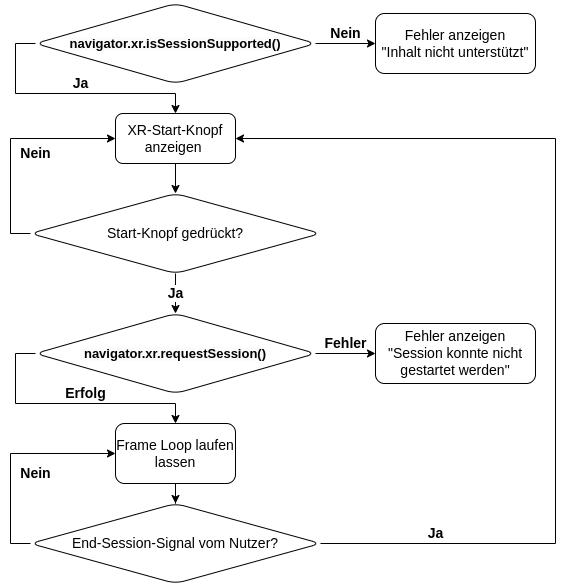
\includegraphics[width=0.5\textwidth]{images/WebXR-App-Flow.png}
    \caption{Application Flow von WebXR-Anwendungen}
    \source{Eigene Darstellung nach \autocite[][Kap. 1.2. Application Flow]{w3c_webxr}}
    \label{fig:webxr-app-flow}
  \end{figure}

Der Flow von WebXR-Anwendungen ist in Abbildung \ref{fig:webxr-app-flow} dargestellt.
Dabei wird zuerst beim Aufrufen der Anwendung geprüft, ob die angegebene Art von XR-Inhalt von der Hardware und dem User Agent (UA) unterstützt werden.
Mit dem User Agent (UA) der Software, ist dabei die Software gemeint, mit welcher der Nutzer auf die Anwendung zugreift, also der Webbrowser des Nutzers.
Ist die Art des XR-Inhalts von der Technik des Nutzers unterstützt, kann die XR-Session vom Nutzer manuell über einen Knopf gestartet werden.
Startet die Session erfolgreich, wird der Frame Loop der Anwendung gestartet.
Der Frame Loop ist eine Schleifenfunktion, die kontinuierlich während der XR-Session ausgeführt wird um die einzelnen Frames, bzw. Bilder, für das XR-Display zu rendern.
Dieser Frame Loop läuft, bis die Session durch den UA beendet wird.
Befindet sich der UA noch auf der Seite der WebXR-Anwendung, wird wieder der Knopf zum Starten der XR-Session angezeigt, falls der Nutzer direkt wieder eine neue Session starten möchte.

\subsection{Three.js}

\subsection{A-Frame}

\subsection{PlayCanvas}

\subsection{Babylon.js}

Babylon.js ist eine Open-Source Rendering- und Game-Engine verpackt in einer JavaScript-Bibliothek die unter Anderem von einem Team von Entwicklern bei Microsoft entwickelt wird.
Es bietet Support für WebGL 1.0/2.0 sowie WebGPU und hat eine Vielzahl von Funktionen, die es Entwicklern ermöglichen, detaillierte 3D-Modelle und -Szenen zu erstellen und zu rendern.
Außerdem bietet es native Unterstützung und eine Dokumentation für WebXR, wodurch die Entwicklung von VR- und AR-Anwendungen vereinfacht wird \autocite[][]{babylon-features}.


\section{Android Debug Bridge}